\documentclass[11pt]{article}

\usepackage{amssymb} % see: http://milde.users.sourceforge.net/LUCR/Math/mathpackages/amssymb-symbols.pdf
\usepackage{mathtools} % for extended mathematical symbols and more

% Page properties :
% See : https://tex.stackexchange.com/questions/36085/latex-without-pages
\usepackage{geometry}
\geometry{margin=16mm}

% To color text :
% see : https://en.wikibooks.org/wiki/LaTeX/Colors
\usepackage[dvipsnames]{xcolor}

% Input file encoding :
\usepackage[utf8]{inputenc}     % makes accents not shit

% To use images : 
\usepackage{graphicx} % use this
\graphicspath{ {./IMG/} } % path midifier for storing images
% to include a picture, type this ('name' is without path or extention) :
% \includegraphics[width=0.5\textwidth]{name}

\usepackage{parskip}

% How to use references :
\usepackage{hyperref} % use this
\hypersetup{
	colorlinks=true,    
	urlcolor=blue,
}

\usepackage{wasysym}

\usepackage{color}

\definecolor{mylightgray}{rgb}{0.95,0.95,0.95}

\usepackage[super]{nth}

% Regulates \tableofcontents max depth
\setcounter{tocdepth}{2}

\usepackage{array}
\newcolumntype{L}[1]{>{\raggedright\let\newline\\\arraybackslash\hspace{0pt}}m{#1}}
\newcolumntype{C}[1]{>{\centering\let\newline\\\arraybackslash\hspace{0pt}}m{#1}}
\newcolumntype{R}[1]{>{\raggedleft\let\newline\\\arraybackslash\hspace{0pt}}m{#1}}
\usepackage{xcolor,colortbl}
\newcolumntype{a}{>{\columncolor{mylightgray}}l}

%% Define a HUGE : https://tex.stackexchange.com/questions/265/fonts-larger-than-huge
\usepackage{fix-cm}   
\makeatletter
\newcommand\HUGE{\@setfontsize\Huge{29}{35}}
\makeatother 

%% Adds padding to tables : https://tex.stackexchange.com/questions/64761/add-just-a-little-more-padding-to-my-table/381439
\usepackage{array}
\setlength\extrarowheight{2pt} % or whatever amount is appropriate


\title{\vspace{15mm}{\HUGE PoGER\footnote{pending name change}}\\
	Vision Document\\
	Version \textit{0.1}}
\author{}
\date{}


% first page
\begin{document}
	

\maketitle


\vspace{30mm}
\begin{center}
	{\Large \textbf{Revisions}}
	\vspace{5mm}
	
	\begin{tabular}{|c|c|c|c|}
		\hline
		\rowcolor{mylightgray}
		\hspace{4mm}\textbf{Date}\hspace{4mm} & \hspace{4mm}\textbf{Version}\hspace{4mm} & \hspace{4mm}\textbf{Description}\hspace{4mm} \\
		\hline
		June \nth{28} 2020 & 0.1 & Initial draft \\
		\hline
		N/A & 1.0 & First Release Placeholder \\
		\hline
	\end{tabular}
\end{center}






\newpage

\begingroup
\hypersetup{linkcolor=black}
\tableofcontents
\endgroup




\newpage

\section{Introduction}

\subsection{Purpose}

This document outlines the vision for the PoGER\footnote{pending name change} project. This includes, but is not limited to :

\begin{itemize}
	\item State the general idea
	
	\item Define high-level features
	
	\item Identify user categories and their respective needs
	
	\item Explore risks and constraints
\end{itemize}


\subsection{Scope}

The scope of this document is limited to this project only. Said project has the following dependencies :
\begin{itemize}
	\item \href{https://www.rpgmakerweb.com/products/programs/rpg-maker-xp}{RPG Maker XP} - The platform on which both following projects run
	
	\item \href{https://essentialsdocs.fandom.com/wiki/Essentials\_Docs\_Wiki}{The Pokemon Essentials project} - The Pokemon "game engine" on RPG maker XP
	
	\item \href{https://pokemon-uranium.fandom.com/wiki/Main\_Page}{The Pokemon Uranium project} - Game built on top of the Pokemon Essentials project
	
	This was chosen as the final test subject for PoGER.
\end{itemize}


\subsection{Definitions, acronyms and abbreviations}
%: Define all terms, acronyms, and abbreviations that are required to interpret the vision correctly. This information might be provided by reference to the project glossary, which can be developed online in the RM repository. 

\begin{itemize}
	\item PoGER\footnotemark[\value{footnote}] - \textbf{Po}kemon Essentials \textbf{G}ame \textbf{E}ngine \textbf{R}ecreation
	
	\item \href{https://en.wikipedia.org/wiki/Game_engine_recreation}{Game Engine Recreation} - In this instance, the process of creating a game engine, in order to play on it games that were developed for another one.
	
	\item RPGXP - RPG Maker XP 
	
	\item PE - Pokemon Essentials
	
	\item Fangame - Fan-made game, or a game that was made by one or multiple people not being employed for that purpose.
	
	\item Dev-time - Quantity of time available to developer(s) to implement this project.
\end{itemize}



\subsection{Preamble}

The first part of this project was a research stage, as a result of which the decision to launch the development of PoGER was made. Most choices about its structure, content and implementation can be traced back to that stage.

At the time of writing, a document detailing the initial research stage doesn't exist yet, but one is planned to be produced shortly.






\newpage
\section{Positioning}

\subsection{Problem Statement}


\begin{tabular}{|a|L{.66\linewidth}|}
	\hline
	The problem of & \begin{itemize}
		\item PE being based on RPGXP, therefore being bound to Windows
		
		\item Performance being poor
		
		\item PE being a convoluted solution to make fangames
		
		\item The need to being fluent in RPGXP-specific Ruby
		
		\item Having no separation between game code and PE code
		
		\item General lack of standards and documentation
		
		\item PE being fan-made and not well maintained
		
		\item Each fangame is isolated, and typically lacks multi-player or online features.
	\end{itemize} \\
	\hline
	affects & \begin{itemize}
		\item Anyone willing to code/coding a fan-game 
		\item People willing to play fangames on other platforms
	\end{itemize} \\
	\hline
	the impact of which is & a variety of unnecessary technical problems \\
	\hline
	A successful solution would be & An implementation of PE that is : \begin{itemize}
		\item performant
		\item available (multi-platform)
		\item straightforward and simpler to develop for
		\item allows to discover fangames
		\item has online capabilities
		\item is separate from the fangames
		\item provides documentation, sets standards
		\item open-source to allow contributors to maintain it
		\item has a way to port games from the original PE
	\end{itemize} \\
	\hline
\end{tabular}


\subsection{Related problem}

This is specific to fangames made using PE.

\begin{tabular}{|a|L{.66\linewidth}|}
\hline
The problem of & fangames using PE typically infringe on the \href{https://www.pokemon.com/us/legal/}{Pokemon IP} \\
\hline
affects & anyone willing to code/coding a fan-game (possibly also players) \\
\hline
the impact of which is & fangame creator typically face legal threats and/or actions \\
\hline
A successful solution would be & to keep a strict position of academic game engine recreation project, with no aim to infringe on IP or provide direction to do so \\
\hline
\end{tabular}



\subsection{Product position statement}

The PoGER project aims to provide a PE implementation that solves the identified problems. The author states that he hasn't been able to identify any similar project.

A secondary objective would be to code a tool capable of helping to port an existing PE-based project.






\newpage 
\section{User Descriptions}

\subsection{User summary}

This may be too straightforward.

\begin{center}
	\begin{tabular}{|C{0.2\hsize}|C{0.3\hsize}|C{0.36\hsize}|}
		\hline
		\rowcolor{mylightgray}
		\textbf{Name} & \textbf{Description} & \textbf{Role}  \\
		\hline
		\textbf{Fangame maker} & Primary end user & Uses PoGER as engine for their game \\
		\hline
		\textbf{Fangame player} & Secondary end user & Plays a game running on PoGER \\
		\hline
		\textbf{Maintainer} & Contributes code to the project & Add functionality, fix bugs, code optimization, etc \\
		\hline
	\end{tabular}
\end{center}

\subsection{User environment}

End users use a number of OS platforms. Targeted platforms are :
\begin{itemize}
	\item Windows (x86)
	\item GNU/Linux (x86)
	\item Android (ARM)
\end{itemize}
Other platfroms may be implemented, like iOS, OSX, PSVita, etc


\begin{center}
	\begin{tabular}{|C{0.2\hsize}|C{0.3\hsize}|C{0.36\hsize}|}
		\hline
		\rowcolor{mylightgray}
		\textbf{Name} & \textbf{Typical platforms}  \\
		\hline
		\textbf{Fangame maker} & Windows, Linux \\
		\hline
		\textbf{Fangame player} & Windows, Linux, Android, etc \\
		\hline
		\textbf{Maintainer} & Windows, Linux \\
		\hline
	\end{tabular}
\end{center}

All targeted platfroms feature online support, which should be leveraged by "nice to have" features.

Touch input (mouse, finger) support looks like a must-have feature.







\newpage
\section{Product Overview}

\subsection{Product perspective}

RPGXP + PE vs PoGER : 
\begin{center}
	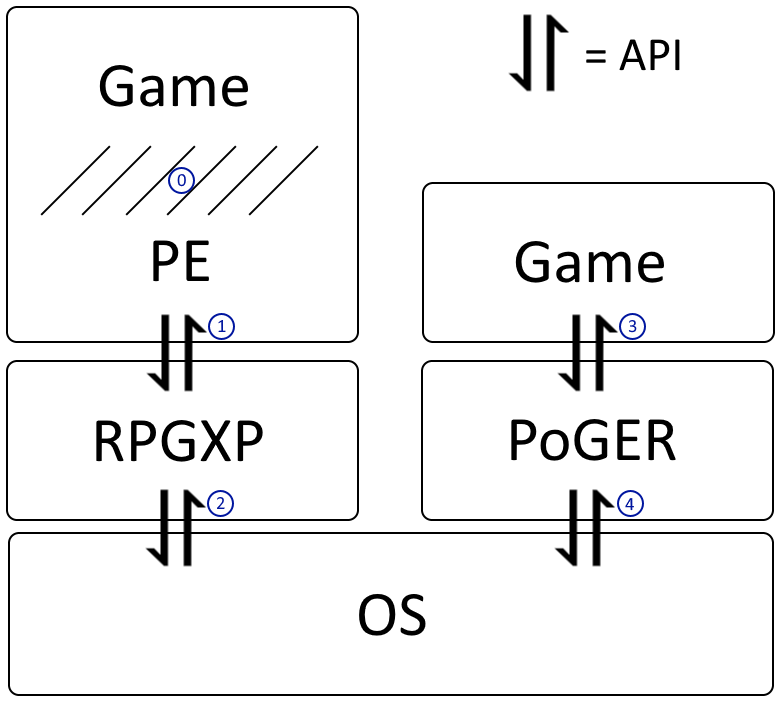
\includegraphics[width=.5\linewidth]{Dia001}
\end{center}

Notes :
\begin{itemize}
	\item[0] - Non-standard, no separation between "game engine" and game code
	\item[1] - Vendor-specific, Ruby language
	\item[2] - Windows-specific, close source
	\item[3] - Standard, clear boudary between game engine and game code
	\item[4] - Platform adaptable, open source, documented API
\end{itemize}

The number of APIs remain constant, but the clearer and more focused structure should allow for better performance, wlĥile bringing desireable features like multi-platform support.


\subsection{Summary of capabilities}

Comparisons are made with regard to RPGXP + PE.

\begin{center}
	\begin{tabular}{|L{.25\textwidth}|L{.7\textwidth}|}
		\hline
		\rowcolor{mylightgray}
		\textbf{User benefit} & \textbf{Feature(s)} \\
		\hline
		Create a game & An end user can create its own game easier, and with less technical knowledge. \\
		\hline
		Focus on content & A game creator doesn't have to understand PoGER implementation details. \\
		\hline
		Ease of collaboration & A PoGER game's structure is modular, optimized for collaborative work. \\
		\hline
		Better performance & With less overhead, an end user experiences less lag and better battery life. \\
		\hline
		Play anywhere & An end user can play on any device which platform is supported. \\
		\hline
		Online features & Online features, like multiplayer, open up possibilities for developers and players. \\
		\hline
		Add functionality & This project is open source. Maintainers and game creators can add functionality they need and everyone benefits from it. \\
		\hline
		Port a game & It should be possible to port a RPGXP+PE game to PoGER. \\
		\hline
	\end{tabular}
\end{center}



\newpage
\section{Product Features}

\subsection{Similar functionality to PE}

As a port of PE, this project should implement similar features and display similar functional behaviour.

\subsection{Easier to develop for}

A game running on PoGER should've the following properties, interesting for developers :
\begin{itemize}
	\item Clear structure, improving collaborative workflow
	\item Separate from game engine
	\item Online capabilities
	\item Platform-agnostic
	\item Documented API
	\item Doesn't require using proprietary/paid software
\end{itemize}

\subsection{Similar functionality to PE}

As a port of PE, this project should implement similar features and display similar functional behaviour.

\subsection{Licensing}

This is an open-source project, inline with free software values. A licensing standard like GNU GPL should be used.













\newpage 
\section{Constraints}

\subsection{Limited dev-time}

This project's initial development is subject to strict time constraints of a few weeks only, with one active developer only.

\subsection{Cross-platform}

Design decisions are to be made with cross-platforming in mind. For example, the choice of programming language is critical for their ease of use and platform compatibility.

\subsection{Original language}

PE was written in RPGXP-specific Ruby, which means none of the source code can be reused. A considerable amount of time will be necessary to re-implement everything.

\subsection{Limited resources}

PoGER targeted platforms may have limited hardware resources (storage, RAM, CPU cores and speed). How much of each is used is to be examined to establish a "\textit{minimum configuration}" and a "\textit{recommended configuration}".

\subsection{Usability}

An end user should not face great usability difficulties, in terms of setting up PoGER, launching it or normally using it.

\subsection{Standards}

Decisions about setting standards, documentation, etc should be made in a straightforward, non-obtuse manner, while being strict enough to be useful without being obstructive.








\vspace{10mm}
\section{Risks}

\subsection{Risk list}

Possible risks to the success of implementation include, but are not limited to :
\begin{itemize}
	\item Lack of dev-time
	\item Unclear or changing goals/requirements of the system
	\item Non-friendly system
	\item Bugs or similar difficulties, which resolution takes significant dev-time
	\item Issues setting up an online infrastructure for online capabilities
	\item Lack of long-term interest. After initial stage, this project could fail to draw interest toward further development.
\end{itemize}







%\newpage 
%\section{Quality ranges and other product requirements}

%TODO









\newpage 
\section{Documentation Requirements}

\subsection{Release notes, README file}

This project is destined to be hosted on a Git-based platform, therefore some form of release notes are nice-to-have's.

Release notes :
\begin{itemize}
	\item Is to be written for each major and minor release of the system.
	\item Should contain a list of changes : additions, removals, changes, bugfixes, etc
	\item Are intended for all end users, therefore should be written \textit{concisely} and with \textit{clear} (but not too complex) language
\end{itemize}

README :
\begin{itemize}
	\item Should exist on the root of the file structure
	\item Should be Markdown-formatted for better readability
	\item Should contain basic information about the project (including links to additional resources), enough for any user to get started
	\item Should contain disclaimers about the nature of this project
\end{itemize}



\subsection{Documentation}

An offline documentation is to be maintained in the \verb|Documentation| folder of the project, both in an editable form and a PDF form. This documentation should be sufficiently structured and complete for any user to be able to answer most common questions and represent most useful details.

Separating documentation into multiple parts seems appropriate :
\begin{itemize}
	\item Installation guides
	\item Primary user documentation
	\item Secondary user documentation
\end{itemize}

Effort should be put to avoid duplicated and outdated informations in these docs.

In combination with READMEs and release notes, it represents a sufficient source of information

\newpage
\section{Others}

\subsection{Buzzwords}
\begin{itemize}
	\item open-source
	\item free software
	\item game engine (recreation)
	\item cooperative
	\item multi-platform
	\item integrated
	\item online capabilities
\end{itemize}

\subsection{Legal disclaimer}

The original author of this project asserts that this is a purely academical endeavor, with no ambition to release this work as a commercial product or part of one. He cannot be held responsible for any use of this project's code or resources outside of its intended purpose.

The author does not condone trademark infringement or any other unlawful act that may involve this project in any way.








\end{document}
